\chapter{Methodology}\label{chap:method}


  \section{Proposed Models } \label{sec:s3}
  
In this section, we present three key contributions aimed at enhancing image splicing detection. Firstly, we introduce the ELA-DenseNet model, a novel fusion of the ELA forensic technique and DenseNet-121 architecture, providing a robust forgery detection system. Secondly, a fine-tuned vision transformer is incorporated to detect and localize manipulated regions in spliced images, harnessing the latest advancements in vision transformer technology. Lastly, a curated dataset of spliced images and corresponding groundtruths is introduced, addressing the critical need for high-quality training and evaluation data. Together, these contributions form a comprehensive and innovative approach to advance image splicing detection, bridging traditional methods with state-of-the-art technologies.

The decision to develop separate models for forgery classification and localization, rather than a unified model for both tasks, is worth noting. It was a deliberate choice driven by a nuanced understanding of the distinct technical demands inherent to each task. Classification entails a comprehensive assessment of the entire image, requiring a model capable of making a binary decision — forged or authentic. This demands the capture of global features and contextual information to discern the overall integrity, aligning well with architectures that are optimized for image classification like CNNs, as exemplified in the ELA-DenseNet model. Conversely, localization zeroes in on specific regions within an image that have undergone manipulation, necessitating a fine-grained analysis. For this task, leveraging object detection and segmentation technologies is crucial to precisely identify manipulated regions, as intricate details such as subtle artifacts and boundary distinctions take precedence. The localization model, therefore, benefits from architectures well-suited for object identification or segmentation, exemplified by the choice of the ViT architecture. This modular approach acknowledges the divergent demands of classification and localization, tailoring each model to excel in its designated role, allowing for more efficient training and task-specific optimization as required by each architecture used.


\subsection{ELA-DenseNet} \label{sec:ss1}

The ELA-DenseNet binary classification model fuses the ELA forensic technique along with a pre-trained DenseNet-121 backbone to determine the authenticity of the query images. The primary aim of the development process was to utilize ELA specifically and then find the optimal CNN architecture that complements it. The model uses a specialized method to apply ELA to the images as a preprocessing step that then returns ELA images in a format similar to Figure \ref{fig:ELA}. These ELA images are given as input to a CNN model. Different CNNs architectures were experimented with, which will be elaborated on in the results section, and the optimal architecture for our use-case was the DenseNet-121. The model was trained on the CASIA V2 dataset for forgery classification. 

\begin{figure}[!h]
    \centering
    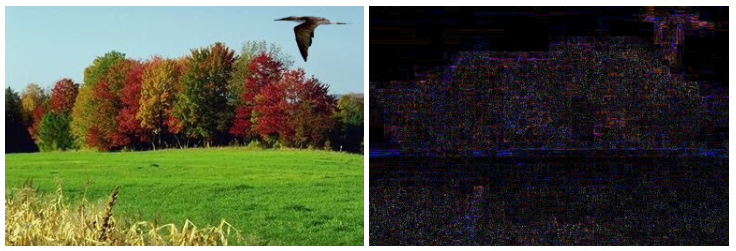
\includegraphics[width=0.8\linewidth]{figures/ELA.png}
    \caption{The left shows a tampered image and the right is its corresponding ELA image}
    \label{fig:ELA}
\end{figure}

DenseNet-121 is a CNN architecture that emphasizes dense connectivity between layers. It introduces the concept of dense blocks, where each layer is connected to every other layer in a feed-forward manner \cite{DenseNet}. This dense connectivity promotes feature reuse and gradient propagation, addressing issues like vanishing gradients. DenseNet-121 consists of convolutional layers, dense blocks, and transition layers. The convolutional layers perform initial feature extraction, while the dense blocks facilitate information flow by concatenating feature maps from previous layers. Transition layers control the number of feature maps and spatial dimensions. Specifically, DenseNet-121 consists of four dense blocks, three transition layers and a total of 121 layers (117-convolution, 3-transition, and 1-classification). It has been successful in image classification tasks. It achieves high accuracy with fewer parameters compared to other architectures \cite{DenseNet}. This parameter efficiency can lead to more compact models and reduced risk of overfitting, especially in situations with limited training data, which is currently the case in image splicing detection.

The tailored model takes a pre-trained DenseNet121 model, unfreezes its layers for fine-tuning, and adds additional layers on top to adapt it for the image splicing detection task. Firstly, it initializes a base model using a pre-trained DenseNet121 model and then loads the pre-trained weights from the ImageNet dataset. The ImageNet dataset is a large visual dataset containing 1,281,167 training images, 50,000 validation images and 100,000 test images. Subsequently, all layers within the base model are set as trainable, enabling fine-tuning during subsequent training. Additional layers are then appended to the base model's output, including a 2D convolutional layer with 1024 filters, a global average pooling layer, a flattening layer, and fully connected dense layers with varied neuron counts and activation functions; ReLU was used throughout the model and softmax was used in the output layer. A dropout layer is incorporated to mitigate overfitting. 

To further prevent overfitting and enhance model training, various configurations were implemented. They include a learning rate scheduler, ReduceLROnPlateau, which dynamically adjusts the learning rate during training based on the validation loss. If the loss plateaus for a certain number of epochs (patience), the learning rate is reduced by a factor of 0.2, with a minimum allowable learning rate. Additionally, early stopping is implemented through EarlyStopping, monitoring validation accuracy and terminating training if no improvement is observed within a specified patience period. The chosen optimizer is RMSprop, a variant of stochastic gradient descent (SGD) that adapts the learning rate for each parameter individually, with a learning rate of 0.0005, a rho parameter of 0.9, epsilon set to 1e-08, and no decay. Finally, the model is compiled using this optimizer, employing binary crossentropy as the loss function and accuracy as the metric for model evaluation during training. The model was set to train for 30 epochs but terminated at the 27th epoch due to the EarlyStopping mechanism. 

\subsection{Fine-tuned Vision Transformer} \label{sec:ss2}

In this proposed method, the aim was to finetune the pretrained IML-ViT \cite{ma2023imlvit} transformer and use its foundational architecture to improve the ability of ViTs to generalize to unseen online images. The motivation for choosing this model lied in its relative simplicity and innovative implementation by the authors who outlined three unique points that they wished to tackle in image manipulation localization tasks: high resolution, multi-scale, and edge supervision. 

In the context of IML, maintaining high resolution is emphasized to address the information-intensive nature of IML tasks, which focus on intricate artifacts rather than object-level macro-semantics. Existing methods, while utilizing various extractors to trace artifacts, often compromise first-hand artifacts through resizing methods. Therefore, preserving the original image resolution is crucial to retain essential details for the model to effectively learn. Additionally, edge supervision becomes paramount in IML as the primary objective is to distinguish between tampered and authentic regions, with a particular emphasis on the boundary of the tampered region. Unlike typical semantic segmentation tasks that identify information within a target region, visible artifacts in IML are concentrated along the periphery of the manipulated region. Consequently, the model is guided to concentrate on learning the distribution of manipulated region edges for optimal performance. Additionally, addressing the variability in tampered area percentages across different IML datasets, incorporating multi-scale supervision during pre-processing and model design stages is deemed essential. This approach helps enhance generalization across diverse datasets with varying proportions of tampered areas, addressing challenges arising from labor-intensive dataset creation and limited sizes in IML datasets such as CASIA V2 and Columbia.

\begin{figure}[!h]
    \centering
    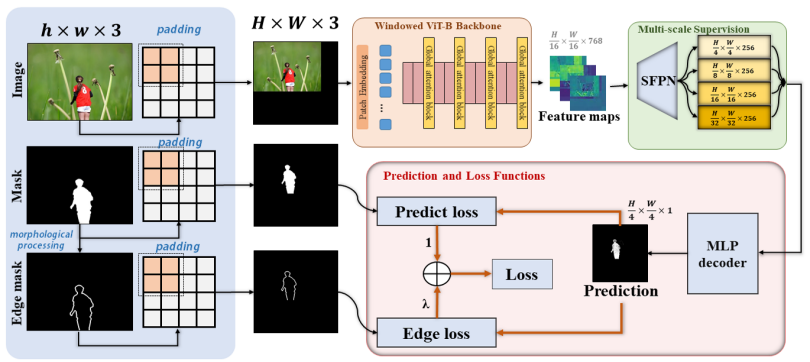
\includegraphics[width=0.75\linewidth]{IMLViT.png}
    \caption{Overview of the general structure of IML-ViT \cite{ma2023imlvit}.}
    \label{fig:imlVIT}
\end{figure}

The model starts with a ViT backbone, which applies self-attention and feed-forward layers to extract meaningful features from the input image. This backbone consists of transformer layers that capture global dependencies and relationships between different parts of the image. After the ViT backbone, a Simple Feature Pyramid Network (FPN) is used to generate a multi-scale representation of the features. The FPN combines features from different scales to capture both fine-grained and high-level information from the image. Next, the features from the FPN are passed through an MLP Predict Head, which consists of fully connected layers that predict the manipulated regions of the image. The output of the MLP is a mask representing manipulated regions, where high values indicate the presence of objects and low values indicate the background. The model computes the loss by comparing the predicted mask to the ground truth mask using Binary Cross Entropy (BCE) loss, and it also introduces an edge loss term to encourage accurate manipulation detection along object edges. To generate the manipulated image, the predicted mask is upsampled using bilinear interpolation, and the manipulated regions are obtained by applying the sigmoid function to the predicted mask.

The available source code for the model was pretrained on the CASIA V2 dataset, meaning another dataset had to be used for fine-tuning. The InTheWild dataset \cite{huh2018fighting} was chosen. It includes 201 spliced images curated from online sources such as THE ONION, a parody (fake) news website, and REDDIT PHOTOSHOP BATTLES, an online community of users who create and share manipulated images.

The fine-tuning process involves adapting the model's parameters to the intricacies of the specific dataset, enabling it to learn and discern patterns indicative of splicing forgeries. By utilizing the learned representations from the pretrained IML-ViT, this method aimed to enhance the accuracy and generalization capabilities of the model, especially to images that typical localization models have proven to not perform well on.

  \section{Proposed Dataset } \label{sec:s3}


In the pursuit of advancing image splicing localization tasks, a main challenge lies in the scarcity of publicly available and representative datasets. Despite efforts to access datasets like the Fantastic Reality Dataset \cite{Kniaz2019ThePW}, attempts to acquire relevant data were hindered by unresponsiveness from dataset authors, underscoring a critical gap in the availability of diverse datasets crucial for training and evaluating models in image splicing detection. Currently available datasets that are popularly used in research in the field are listed in Table \ref{table:datasets}. InTheWild, the selected dataset for fine-tuning the ViT model, designed for an online-centric use-case, is suitable but constrained by its small size. Recognizing the inadequacy of the existing dataset, there emerged a compelling need to expand upon it. This imperative stemmed from the necessity to augment the dataset's diversity and size, ensuring a more robust foundation for refining models tailored to the challenges of online image manipulation scenarios. To address this, the proposed dataset, an expansion of the InTheWild dataset \cite{huh2018fighting}, was curated, providing a larger training dataset for fine-tuning the ViT. The objective was to enhance the ViT's ability to generalize by incorporating a representative and diverse dataset from multiple creators, reflecting samples encountered realistically online.

With the primary goal of expanding the dataset, we sourced the 208 additional images from the same online platforms, namely THE ONION and REDDIT PHOTOSHOP BATTLES. This approach aimed to uphold the dataset's homogeneity. However, with the aim of grater representation, the new images display a greater variety of post-processing and more complex subject matters and even different visual styles. The incorporation of these new images resulted in more than doubling the size of the initial dataset from 201 to 409. Since no groundtruth masks exist for online images, manual annotations were performed, and the corresponding groundtruth masks were created using Labelbox, with a specific emphasis on leveraging their advanced AutoSegment 2.0 feature. The new dataset was labeled ExpandedInTheWild. Figure \ref{fig:expanded} displays samples along with their groundtruth masks.

\begin{figure}[!h]
    \centering
    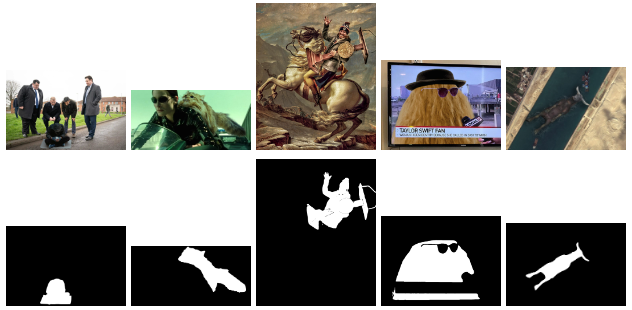
\includegraphics[width=0.75\linewidth]{EITW.png}
    \caption{Samples from the curated ExpandedInTheWild dataset}
    \label{fig:expanded}
\end{figure}

\begin{table}[]
\centering
\renewcommand{\arraystretch}{1.7}
\begin{tabular}{|p{2.2cm}|p{1.8cm}|p{2cm}|p{1.5cm}|p{2.5cm}|}
\hline
Dataset Name & Forgery Type & Real/Forged Images & Image Format & Post-processing \\ \hline
CASIA V1 & Splicing, copy move, removal & 800/921 & TIFF, JPEG, BMP & No \\ \hline
CASIA V2 & Splicing, copy move, removal & 7491/5123 & TIFF, JPEG, BMP & Yes \\\hline
Columbia Grey & Splicing & 933/912 & BMP & No \\\hline
Columbia Color & Splicing & 183/180 & TIFF & No \\\hline
Carvalho & Splicing & 100/100 & PNG & Yes \\\hline
IMD2020 & Splicing, copy move, removal & 35000/35000 & JPEG & Yes \\\hline
Dresden & Splicing, copy move, removal & -/16961 & JPEG & No \\\hline
Fantastic Reality & Splicing & 12000/1000 & JPEG & Yes \\\hline
Realistic Tampering & Object insertion, removal & 220/220 & TIFF & Yes \\\hline
DEFACTO & Splicing, copy move, removal & -/229000 & JPEG, PNG, TIFF & Yes \\\hline
InTheWild & Splicing, copy move, removal & -/201 & JPEG, PNG & Yes \\\hline
\end{tabular}
\caption{Available image forgery detection datasets}
\label{table:datasets}
\end{table}



